\section{Detector Installation}
\label{sec:fdsp-tc-inst}

\subsection{Introduction}
\label{sec:fdsp-tc-inst-intro}

The DUNE detector installation will proceed in three phases the CUC setup phase, the installation setup phase, and the detector installation phase. The CUC setup phase is the first step in the installation process. The start of the CUC setup phase begins when the underground area for the North Cavern and Central Cavern become available to LBNF and DUNE. At this time the cryostat construction can begin in The North Cavern and equipment installation can begin in the Central Cavern or the Central Utility Cavern (CUC). The main equipment from DUNE which is installed in this phase is the equipment in the DUNE dataroom. The detector installation setup phase begins during the cryostat membrane installation period. In this phase the equipment needed to perform the detector installation will be erected in North Cavern. This includes the installation of the bridge across the cavern, the installation cleanroom, lifting equipment and work platforms, the cold boxes and cryogenic system for testing APA, and the DSS with related switchyard. In the third phase of the installation the detector itself will be installed. The work in each phase will be described the following sections.

\begin{dunefigure}[Layout of the underground area]{fig:cavern-layout}
  {Top view of the layout at the 4850 level at SURF. Shown are the 3 large excavations and the location of detectors in excavation \#1 and \#3. Excavation \#2 is the CUC which houses the DUNE dataroom and the underground utilities.}
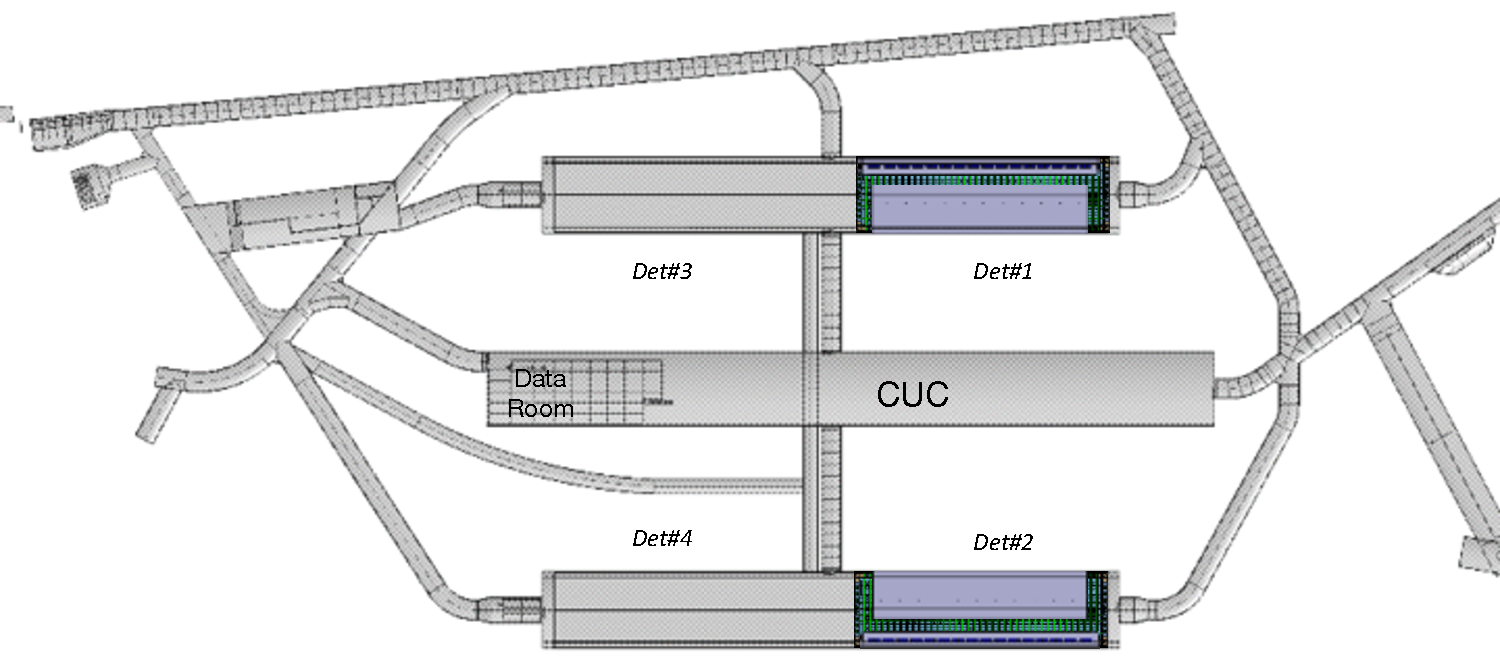
\includegraphics[width=.9\textwidth]{cavern-layout}
\end{dunefigure}

\fixme{insert very simple schedule}

%%%%%%%%%%%%%%%%%%%%%%%%%%%%
\subsection{Installation Process Description}
\label{sec:fdsp-tc-inst-proc}

\subsubsection{CUC Installation Phase}

\begin{dunefigure}[Layout of the DUNE dataroom and experimental workarea in CUC]{fig:install-cuc}
  {TOP: The overall layout of the DUNE spaces in the CUC is shown. The inner room is the DUNE dataroom which houses the underground computing and the outer area referred to as the experimental workarea is a general purpose workarea. Bottom: The first row of racks in the data room is shown. The first two racks are the  CF interface racks. The image was taken from the ARUP design drawing U1-FD-T-701}
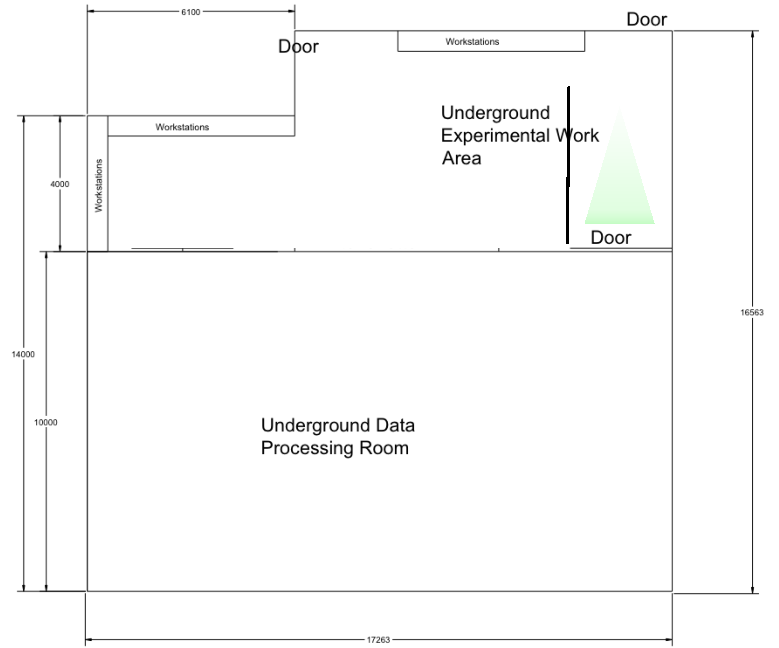
\includegraphics[width=.7\textwidth]{cuc-layout}
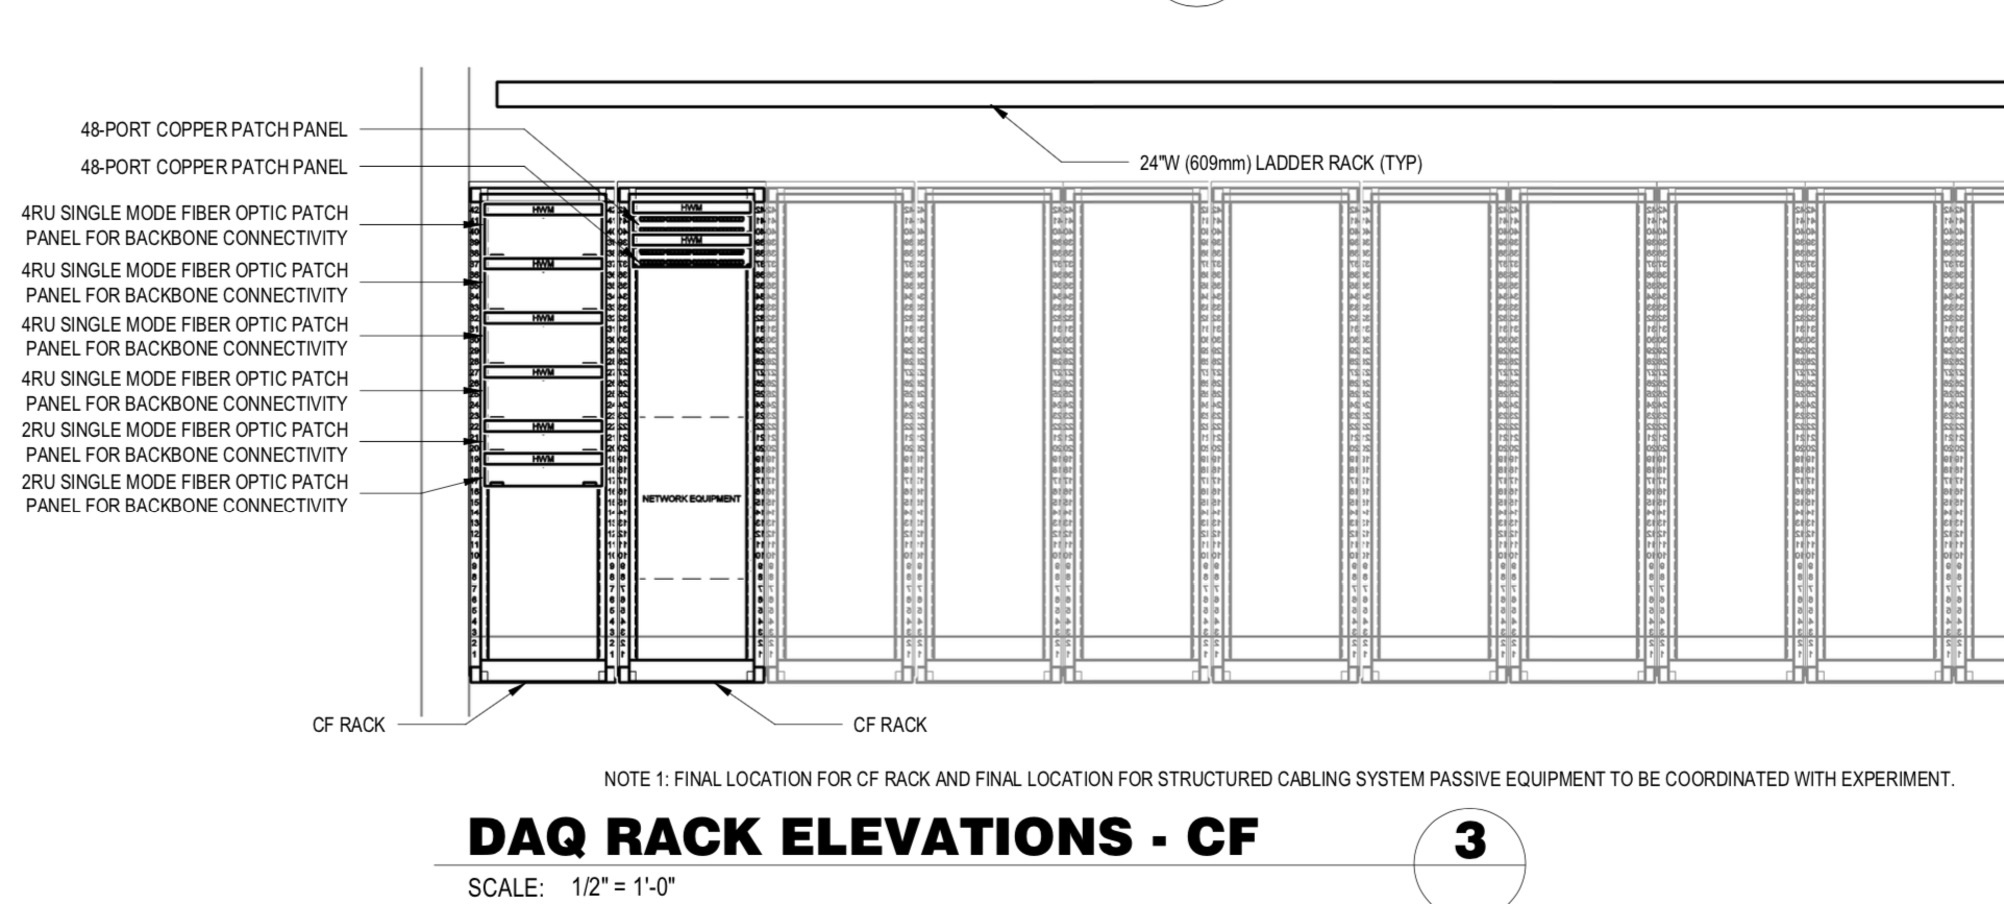
\includegraphics[width=.9\textwidth]{cuc-cf-racks}
\fixme{need to use a figure from the 90\% submittal}
\end{dunefigure}


The first stage of the CF work ends when the outfitting of 
the North and Central caverns is complete. At this time the CUC is ready for DUNE outfitting and the cryostat installation can start for detector 1. During this period DUNE will not have assess to the detector excavations as the heavy steel work for the cryostat will be ongoing. The only work planned for DUNE in this period is the outfitting of the data room and work area room in the CUC shown in Figure \ref{fig:install-cuc}. CF will provide the empty room with an 18 in false floor, a 500KVA power disconnect, and connections for chilled water sufficient to cool the racks. The dataroom like the adjacent CF electronics room will be outfitted with a dry fire extinguishing system. 

The water cooled racks, cable trays, power distribution, and water distribution are the responsibility of DUNE and will be installed once the space becomes available. The installation of the racks needs to be coordinated with CF as the first two racks are for CF usage and need to be in place before the underground phase one work is complete. Some small overlap will be needed between CF and DUNE at this time.

At the same time the eight DAQ racks which receive the data from the underground area and then transmit the data to FNAL will also be installed. With this infrastructure in place the DAQ group can begin constructing and testing the final DUNE DAQ.  

The underground experimental work area is a general purpose area that will need to serve many purposes during the DUNE installation. Initially the area will be outfitted with office equipment for the installation team, workstations for DAQ, and a basic conference area for meetings.  The room is 4-6.4 \si{m} deep and 20 \si{m} long so it can serve several functions.

During this early installation stage the machine shop and DUNE storage area will also be setup in the detector excavation area.

\subsubsection{Installation Setup Phase}

Once the steel structure of the cryostat is complete the remaining work will be focused inside the cryostat. 
There will still be a lot of activity outside the cryostat as the 4,000 crates of foam and other materials are transported inside but the outer structure will be in position so some DUNE work can start. 
The first piece of equipment to installed will be the bridge between the North and South drifts. 
This will allow the cryogenics equipment to travel from the North drift to the CUC and will provide part of the structure for the cleanroom. 
Construction of the cleanroom frame and related hoisting equipment can then begin. 
The largest most complex equipment that must be constructed in this phase are the cold boxes and related cryogenics system. 
Due to the size of the cold boxes these must be constructed in place. 
The layout of the installation region outside the cryostat is shown in Figure \ref{fig:install-ug-layout}. 
This figure shows a cut below the bridge so the majority of the installation equipment can be seen. 
The three 15 \si{m}tall cold boxes are seen in blue next to the yellow access stairway. 

The hoisting equipment and the rail system needed to move the detector components in the installation area interfaces with the bridge, cryostat and possibly the cleanroom mechanical structure. 
Installing this early will make transporting equipment around the area outside the cryostat significantly simpler. 
\fixme{Do we want a figure of just the rails and switchyard?} 
The assembly towers for the APA assembly, APA cabling, and CPA assembly can be installed when it is most convent for the cryostat installation crew. 
Just prior to the start of detector installation the cleanroom walls will be installed, the area will be cleaned and added filters will be installed to convert the area to an ISO-8 cleanroom.

During this phase of the cryostat installation the majority of the cryostat work will be inside an at the 4910 level. 
This will allow significant work to be performed on the cryostat roof for the cryogenic system installation and the detector installation setup. 
The cryostat crossing tubes will be installed on the roof 
\fixme{figure of the cryostat crossing tube with the mechanical connection to the I-beams and the inteface to the membrane.} . 
These assemblies are welded to the 1 \si{cm} thick steel cryostat roof and are then additionally cross braces to the large I-Beams. 
The thick walled tubes which penetrate through the foam insulation are in place at this time. 
Once the crossing tubes are in place the large tees for the cold electronics can be installed. 
The next step in the installation requires the internal roof of the cryostat to be complete. 
At this time the DSS support feedthrus can be installed and possible the DSS beams can be lifted into positions. 
The details of how to coordinate this work will be iterated with the cryostat manufacturers as the design work is completed. 
At this time the cold electronics mechanical feedthrus can be installed. 
Once work on the feedthru are complete then the mezzanines for the cryogenic system and the detector electronics racks can be installed.
Finally the cable trays,  piping, lighting, and cryostat roof flooring are installed. 
At this time the cryostat roof is ready for the start of the DAQ installation in the detector area.

The last steps in the installation setup phase is the installation of the cryostat internal piping, cleaning the cryostat, installing the false floor, and filtered lighting to protect the photon detectors. 
\fixme{ Insert the figure of the piping inside the cryostat. }



\subsubsection{Detector Installation Phase}

At the start of the detector installation phase the work on the cleanroom is complete, the DSS is installed in the cryostat including the switchyard near the TCO. 
The light in the cryostat and cleanroom will be filtered to protect the photon detectors and the air will be filled to reduce the dust collected during installation. 
The cryogenic piping will be in place along with the false floor. 
The false floor both gives a flat work area and protects the 1.2 \si{mm} thick stainless steel cryostat membrane. 



The first detector equipment to be installed is the CISC thermometers and cameras at the East end of the cryostat which will be used to monitor the cool down, filling and commissioning of the detector. As these componets are snall the installation work can be performed using a scissor lift with 12 \si{m} reach. 
At present this is the tallest battery operated (thus cleanroom compatable) scissor lift available.
The next step in detector installation is the field cage end-wall installation. 
The endwall panel will be brought underground as slung loads in transport crates holding 4 end-wall panels each. The crates will be stored in the West end of the North cavern in preeparation for installation. 
The crates will be brought to the material airlock using a pallet jack,  the outer layer of packaing is removed and the inner packaging cleaned.
A clean forklfit is then used to put 



In an effort to get an early estimate of the equipment required to
install the detectors the \dword{uit} has developed a preliminary
installation plan that outlines the installation process. At present the installation plan consists of a \threed model of the cryostat in the excavations. The \dword{spmod} elements are inserted in the model and a proposal for how they are transported, assembled, and inserted into the cryostat has been conceptually developed and expressed in a series of images some of which are shown in Figures~\ref{fig:Install-seq} and~\ref{fig:cpa-fc-unpack-assy}. 
%
Conceptual designs of the infrastructure needed to support
the transport and assembly are also included in the model. See Figures~\ref{fig:Install-ISO-Top} and~\ref{fig:Install-TopView}. With this
as a tool, the proposed installation sequence can be iterated with the
consortia to converge on a baseline installation plan. A similar
process will be followed for the \dword{dpmod} once the base
configuration for the \dword{sp} installation is agreed upon. The
\dword{uit} has focused initially on the \dword{spmod} as the
\dword{sp} components are larger and the installation process more
complex. 

\begin{dunefigure}[APA and CPA installation steps]{fig:Install-seq}
  {Top row from left:  crated \dword{apa} rotating to vertical position;  crated vertical \dword{apa} placed in cart; \dword{apa} panels moved to fixture using the under-bridge crane. Bottom row: series showing \dword{cpa} panels uncrated and moved to fixture. }
%\includegraphics[width=.9\textwidth]{apa-install-seq-top}
%\includegraphics[width=.9\textwidth]{cpa-install-seq-bot}
\end{dunefigure}

\begin{dunefigure}[\dword{cpa} and \dword{fc} unpacking and assembly]{fig:cpa-fc-unpack-assy}
  {On the left, the assembled \dword{cpa} panel is placed onto the north \dword{tco} beam. On the right, the (green) \dword{fc} panels (already lowered into \dword{sas} and moved into the clean room) are installed as the \dword{cpa} array hangs under the \dword{tco} beam. }
%\includegraphics[width=.9\textwidth]{cpa-fc-unpack-assy}
\end{dunefigure}

\begin{dunefigure}[\threed model of underground area showing installation infrastructure]{fig:Install-ISO-Top}
  {\threed model of the underground area showing the infrastructure to install the \dword{spmod} in cryostat~1. The most significant features are presented including the \dword{apa} and \dword{cpa} assembly areas, the region around the \dword{tco} for materials entering the cryostat,  the changing room, the region for the materials air lock, (\dword{sas}), 
  and the means of egress.}
%\includegraphics[width=.9\textwidth]{Install-ISO-Top}
\end{dunefigure}

\begin{dunefigure}[Section view of the \threed model showing layout]{fig:Install-TopView}
  {Section view of the \threed model showing layout, looking down on the installation area from below the bridge. Areas shown, left to right,  are the cryostat and \dword{tco}, the platform in front of the \dword{tco}, the dressing area, the \dword{apa} and \dword{cpa} assembly area (directly under the bridge), and the stairs and elevator. The lower right corner of the region is used as the materials air lock.}
%\includegraphics[width=.9\textwidth]{Install-TopView}
\end{dunefigure}





%The current installation plan is described. 
In the current installation plan, \dword{dune} will take
ownership of the different underground areas at different times. The
surface data room and the underground room in the \dword{cuc} are available
significantly before the collaboration has access to the cryostats; 
the optical fibers between the surface and underground will be in
place even earlier. This will allow a \dword{daq} prototype to be developed
and tested early. The installation of the \dword{daq} hardware can also be
finished before the start of detector installation if desired, so the
\dword{daq} will not be on the critical path.  When the collaboration receives
access to Cryostat~1 the steel work for Cryostat~2 will be
finished and the work on installing the membrane will have
started. Excavation will be complete.  For planning purposes it is
assumed that the first \dword{detmodule} will be \dword{sp} and the second
\dword{dp}. The first step in the \dword{sp} installation is to
install the cryogenics piping and the \dword{dss}. As this piping will
require welding and grinding, it is a dirty process and must be
complete before the area can be used as a clean room. When this is
complete the cryostat can be cleaned and the false floor
re-installed. The clean infrastructure for installing the \dword{detmodule},
including the clean room, work platforms, scaffolding, the
fixturing to hold the detector elements during assembly, and all the
lifts need to be set up. Once the infrastructure is in place and the
area is clean, the installation of the main elements can start. The
general layout of the installation area showing the necessary space
and equipment is shown in Figure~\ref{fig:Install-seq}. 

The \dword{spmod}  is installed by first installing the west endwall or
endwall~1 (see Figure~\ref{fig:endwall}).

\begin{dunefigure}[End view of \dword{spmod} with \dword{ewfc} in
  place]{fig:endwall}
  {End view of \dword{spmod} with \dword{ewfc} in
  place, with one row of \dwords{apa} and \dwords{cpa}.}
%\includegraphics[width=0.6\textwidth]{endwall.png}
\end{dunefigure}

The \dwords{apa} and \dwords{cpa} with top and bottom \dword{fc} panels are
installed next. The plan is to install six \dwords{apa} and four
\dwords{cpa} per week, which is enough to complete one of the \num{25}
rows every week. Additional time is built into the schedule to take
into account that the installation will be slower at the beginning and
some re-work may be needed. By building west-to-east, complete rows can
be finished and tested before moving to the next row. This reduces the
risk of finding a fault after final \dword{fc} deployment and cabling,
which would require dismantling part of the \dword{detmodule}. Some of the steps
needed to install the \dword{apa} and \dword{cpa} modules outside the
cryostat are also shown in Figure~\ref{fig:Install-seq}.  The middle three
panels show how the \dword{apa} needs to be handled in order to rotate
it and mount it to the assembly frame. After two \dwords{apa} are
mounted on top of each other, the cabling for the lower \dwords{apa}, and the
\dword{ce} and \dword{pd} cables can be installed. The
lower three panels show how the \SI{2}{m} \dword{cpa} sub-panels are
removed form the transport crates and assembled on a holding frame. Once
the \dword{cpa} module is assembled the \dword{fc} units can be
mounted. Finally, once the \dwords{apa} and \dwords{cpa} are installed,
the endwall~2 can be installed. A high-level summary of the schedule
is shown in Figure~\ref{fig:Install-Schedule}.

\begin{dunefigure}[High-level installation schedule]{fig:Install-Schedule}
  {High-level installation schedule.}
 %\includegraphics[width=\textwidth]{TP-Schedule-Feb2018.pdf}
\end{dunefigure}


 Installation Coordination and Support %or 
(also called simply \textit{Installation}) is
responsible for coordinating the detector installations, providing
detector installation support and providing installation-related
infrastructure. The installation group management responsibility is
shared by a scientific lead and a technical lead that report to the
Technical Coordinator. The %underground 
group responsible for activities in the underground areas is referred to as
the \dword{uit}. The \dword{itf} group, which delivers equipment to the
Ross Shaft, and the \dword{uit}, which receives the equipment
underground, need to be in close communication and work closely
together.

Underground installation is in general responsible for coordinating
and supporting the installation of the \dwords{detmodule} and providing
necessary infrastructure for installation of the experiment. While the
individual consortia are responsible for the installation of their own
detector equipment, it is essential that the detector installation be
planned as a whole and that a single group coordinates the
installation and adapts the plans throughout the installation
process. The \dword{uit} has responsibility for overall coordination
of the installations. In conjunction with each consortium the
\dword{uit} makes the installation plan that describes how the
\dwords{detmodule} are to be installed. The installation plan is used to define
the spaces and infrastructure that will be needed to install them.
%detectors. 
The installation plan will also be used to define the
interfaces between the Installation group and the consortium
deliverables.

For the \dwords{detmodule} to be installed in safe and efficient
manner, the efforts of the individual consortia must be coordinated
such that the installation is planned as a coherent process. The
interfaces between the individual components must be understood
and the spaces required for the installation process planned and
documented. The installation planning must take into account the
plans and scope of the \dword{lbnf} effort and the individual plans of
the nine consortia. By working with the \dword{lbnf} team and the
members of the consortia responsible for building and installing their
components, a joint installation plan and schedule, taking into account
all activities and needs of all stakeholders, can be developed. Although
the organization of the installation effort is still evolving, 
an installation coordinator will be the equivalent of a scientific lead for this effort.

One of the primary early responsibilities of the \dword{uit} is to
develop and maintain the \dword{dune} installation plan and the
installation schedule. This installation plan 
describes the installation process in sufficient detail to demonstrate
how all the individual consortium installation plans mesh and it 
gives an overview of the installation process. The installation plan
is used by the \dword{uit} to define the underground infrastructure
needed for detector installation and the interfaces it has with respect  to 
the consortia. The \dword{uit} is responsible for reviewing and
approving the consortium installation plans. Approved installation
plans, engineering design notes, signed final drawings, and safety
documentation and procedures are all prerequisites for the \dword{prr}. 
Approved procedures, safety approval, and
proper training are all required before the \dword{uit} performs
work. During the installation phase the installation leadership 
coordinates the \dword{dune} installation effort and adapts the schedule
as needed. The installation coordinator, together with management, will also
resolve issues when problems occur.




%%%%%%%%%%%%%%%%%%%%%%%%%%%%
\subsection{Transition to Commissioning}
\label{sec:fdsp-tc-inst-commiss}

After the \dwords{detmodule} are installed in the cryostats there remains a lot
of work before they can be operated. First the \dword{tco}
must be closed. This requires bringing back the cryostat manufacturer. 
First the missing panel with the steel beams
and steel panel are installed to complete the cryostat's outer
structural hull. Then the remaining foam blocks and membrane panels
are installed from the inside using the roof access holes 
to enter the cryostat. 

In parallel, the \lar pumps are installed at
the ends of the cryostat and final connections are made to the
recirculation plant. Once the pumps are installed, the cryostat is
closed, and everything is leak tested, the cryogenics plant can be
brought into operation. First the air inside the cryostat is purged by
injecting pure argon gas at the bottom %of the detector 
at a rate such
that the %detector 
cryostat volume is filled uniformly but faster than the diffusion
rate. This produces a column of argon gas that rises through the volume %detector
and sweeps out the air. This process is referred to as the \textit{piston
purge}. When the piston purge is complete the cool-down of the \dword{detmodule}
can begin. Misting nozzles inject a liquid-gas mix into the cryostat
that cools the detector components at a controlled rate. 

Once the detector is
cold the filling process can begin. Gaseous argon stored at the surface 
at \surf is brought down the shaft and is re-condensed underground. The \lar then flows through filters to remove any H$_2$O or O$_2$ and
flows into the cryostat. Given the very large volume of the cryostats
and the limited cooling power for re-condensing, it is  %the liquid is
expected to take \num{12} months to fill the first \dword{detmodule} and \num{14} months to
fill the second. During this time the detector readout electronics
will be on monitoring the status of the detector. % so the status of the detector can be monitored. 
Once the
\dword{detmodule} is full, the drift high voltage can be carefully ramped up and
data taking can begin.

%%%%%%%%%%%%%%%%%%%%%%%%%%%%
\subsection{Installation Infrastructure}

The installation scope includes the infrastructure needed to install
the \dword{fd} such as the cleanroom, a small machine shop, special
cranes, scissor lifts, and access equipment.  Additional equipment
required for installation includes: rigging equipment, hand tools,
diagnostic equipment (including oscilloscopes, network analyzers, and
leak detectors), local storage with some critical supplies and some
personal protective equipment (PPE). The \dword{uit} will also provide
trained personnel to operate the installation infrastructure. The
consortia will provide the detector elements and custom tooling and
fixtures as required to install their detector components.





%%%%%%%%%%%%%%%%%%%%%%%%%%%%
\subsection{Prototyping and Testing (QA/QC)}
\label{sec:fdsp-tc-inst-qaqc}

\fixme{QA/QC Prototyping and testing}
\fixme{Include requirements; Lessons learned from ProtoDUNE-SP}


These will set the schedule for the installation and will
determine the planning for staffing and budget. Having good estimates
for the time needed and having enough experience to ensure that the
interfaces are understood and the procedures are complete is important
for accurate planning. The experience at \dword{protodune} will be
very important as the \dword{protodune} installation establishes the
procedures for handling all the detector elements and in many cases
gives accurate estimates for the time needed. However, in the case of
the \dword{spmod}, many of these procedures need to revised or
newly developed. For example, the \dword{spmod} will be twice as high as
\dword{pdsp}, so two \dwords{apa} need to be assembled together
and a totally different cabling scheme is needed. Testing the
cabling must be done prior to the \dword{tdr} %as this is needed 
in order to
ensure the design is viable. The \dword{dp} will also need to develop
installation procedures as the \dword{dpmod} 
will have a significantly different \dword{fc} and cathode plane. 

By definition, the installation  is on the critical path, making it vital
that the work be performed efficiently and in a manner that has low
risk. In order to achieve this, a prototype of the installation
equipment for the \dword{spmod}  will be constructed at Ash
River (the \nova neutrino experiment \dword{fd} site in Ash River, Minnesota, USA), and the installation process tested with dummy detector
elements. It is expected that the setup will be available at the time
of the \dword{tdr}, but any lessons learned will need to be implemented and
tested after this. In the period just prior to the start of
installation, the Ash River setup will be used as a training ground for
the \dword{uit}.




%%%%%%%%%%%%%%%%%%%%%%%%%%%%
\subsection{Safety}
\label{sec:fdsp-tc-inst-safety}


%%%%%%%%%%%%%%%%%%%%%%%%%%%%
\subsection{Costs, Schedule and Risk Analysis}
\label{sec:fdsp-tc-inst-cost}

\subsection{Conclusions}
\label{sec:fdsp-tc-inst-concl}



The installation infrastructure to be provided by the \dword{uit}
includes: the underground ISO 8 (or class \num{100000}) clean room
used for the installation; cranes and hoists (if they are not
delivered by \dword{lbnf}); and scissor lifts, aerial lifts, and the common
work platforms outside the cryostat. The \dword{uit} will have
responsibility for operating this equipment and assisting the
consortia with activities related to rigging, material transport, and
logistics. Each consortium is responsible for the installation of
their own equipment, so the responsibility of the installation group is
limited, but the material handling scope is substantial. To support
the installation process, an installation floor manager will lead a
trained crew with the main responsibility of transporting the
equipment to the necessary location and operating the cranes, hoists,
and other common equipment needed for the installation. It is expected
that the installation crew will work with the teams from the various
consortia but will mainly act in a supporting function. The
\dword{uit} floor manager will be responsible for supervising the
\dword{uit} crew, but the ultimate responsibility for all detector
components remains with the consortia even while the underground
team is rigging or transporting these components.  This will be
critical in the case where any parts are damaged during transport or installation,
as the consortia need to judge the necessary actions. 
\fixme{judge the situation and determine the necessary actions?}
For this reason,
a representative or point of contact (POC) from the consortia must be
present when any work is performed on their equipment. The consortium
is responsible for certifying that each installation step is properly
performed.

The \dword{uit} acts as the primary point of contact with
\dword{lbnf} and \surf from the time the components reach the Ross
headframe until the equipment reaches the experimental cavern. If
something goes wrong, \surf calls the \dword{uit} leader who then
contacts the responsible party. The consortia are responsible for
delivering to the \dword{uit} all approved procedures and specialized
tooling required for transport. The \dword{uit} leader acts as a point
of contact if the \dword{lbnf} or \surf team has questions or difficulties
with the underground transport.  The \dword{uit} receives the
materials from \dword{lbnf} and \surf at the entrance to the \dword{dune}
excavations. The \dword{uit} then delivers the equipment to the
required underground location.

